\documentclass[tikz,border=12pt]{standalone}
\usepackage{pgfplots}
\pgfplotsset{compat=1.18}

\definecolor{curveblue}{HTML}{1971C2}
\definecolor{generatorpink}{HTML}{C2255C}
\definecolor{gridgray}{HTML}{DEE2E6}

\begin{document}
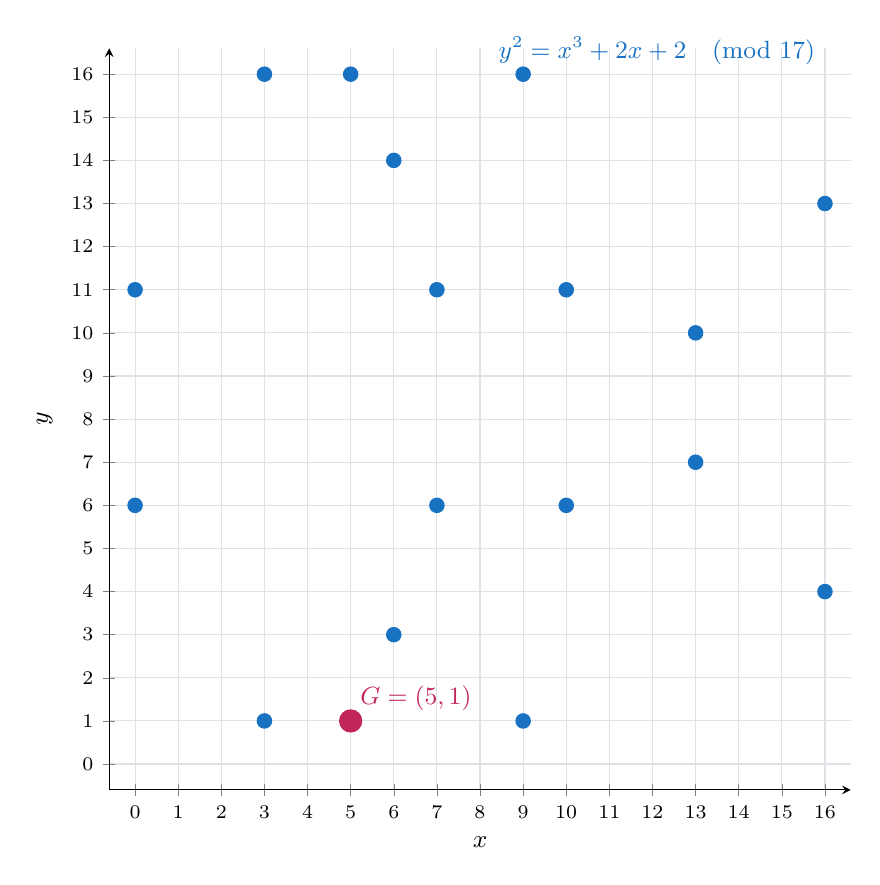
\begin{tikzpicture}
  \begin{axis}[
    width=11cm,
    height=11cm,
    xmin=-0.6,
    xmax=16.6,
    ymin=-0.6,
    ymax=16.6,
    axis lines=left,
    axis equal image,
    xtick={0,...,16},
    ytick={0,...,16},
    grid=both,
    grid style={gridgray},
    tick label style={font=\scriptsize},
    xlabel={$x$},
    ylabel={$y$},
    label style={font=\small},
    clip=false
  ]
    \addplot[only marks, mark=*, mark size=2.6pt, curveblue]
      coordinates {
        (0,6) (0,11) (3,1) (3,16) (5,16) (6,3) (6,14)
        (7,6) (7,11) (9,1) (9,16) (10,6) (10,11)
        (13,7) (13,10) (16,4) (16,13)
      };
    \addplot[only marks, mark=*, mark size=4pt, generatorpink]
      coordinates {(5,1)};
    \node[anchor=south west, text=generatorpink, font=\small]
      at (axis cs:5,1) {$G=(5,1)$};
    \node[anchor=south east, text=curveblue, font=\small]
      at (axis cs:16,16) {$y^2=x^3+2x+2 \pmod {17}$};
  \end{axis}
\end{tikzpicture}
\end{document}
